% !TeX program = xelatex
% 接在 3.5 之後，沿用既有論文主檔。

% ==================================================
% 3.6 移動中操作與機構約束控制
% ==================================================
\section{移動中操作與機構約束控制}
\label{sec:mobile_constrained_operation}

移動中操作需要協調底盤進度、末端追蹤與物件互動。Burgess-Limerick 等人\cite{burgess2023motm}以移動與操作重疊改善多步驟任務的執行效率；對門與抽屜等關節式物件，則需進一步考量機構運動與全身構型的相容性\cite{mittal2022articulated}。本節以共用全身控制核心承接不同任務參考，說明抓持條件、機構約束及持物狀態的切換。


% ==================================================
% 3.6.1 移動中接近與抓持條件
% ==================================================
\subsection{移動中接近與抓持條件}
\label{subsec:moving_approach_grasp}

物件尚未抓持時，末端目標以世界座標表示。即使底盤持續移動，手臂仍需配合補償底盤造成的相對位移，使 TCP 接近物件。抓取階段依物件外形設定位置容許區域、姿態誤差及適用的相對速度條件；固定橫桿把手另檢查沿夾爪開合軸的誤差。

圓柱的移動中接近採用第 3.5.4 節之距離展開及後段併線，底盤逐軸限速與手臂進度的關係見\cref{fig:ch3_mobile_approach_distance_profile}。底盤可在接近與閉爪期間繼續行進，手臂則以世界座標抓取目標補償其運動；抓持成立後，再依抬升及運送階段更新為適用的底盤相對參考。

閉爪時機由接近進度與狀態判定。目前模擬利用模擬器提供的手指位置與接觸力資訊確認抓持，不將閉爪命令回傳成功視為夾持成功。以 $\gamma_f(t)\in\{0,1\}$ 表示該任務的抓持證據判定，要求
\begin{equation}
    \gamma_f(t)=1,
    \qquad
    t\in[t_b-T_{\mathrm{ev}},t_b],
    \label{eq:ch3_grasp_evidence_duration}
\end{equation}
其中 $T_{\mathrm{ev}}$ 為確認時間，$t_b$ 為判定成立時刻。手指位置、接觸力及持續時間的門檻依物件類型設定，並於第四章揭露。移動中抓取另受可達時間窗約束，錯過時依既定策略重新接近或轉為收斂抓取，並記錄原移動中操作未完成的原因。

目前模擬在抓持證據成立後，依任務使用夾爪與物件間的理想固定連接。連接建立與解除皆由執行端回報確認，控制器再更新抓持狀態。此假設用於研究抓持後的協同運動，其影響於第四章的限制分析說明。上述手指狀態與接觸力為模擬資訊；實機部署須另以視覺觀測或外加感測器建立對應的抓持確認機制。

% ==================================================
% 3.6.1 接近、閉爪確認與抓持成立之狀態轉移
% ==================================================
抓持狀態的轉移如\cref{fig:ch3_grasp_state_transition}所示。閉爪命令發出後，需檢查手指位置與接觸證據，待條件持續成立並取得必要的連接確認後，才銜接抓持後的機構操作或持物運送。

\begin{figure}[htbp]
    \centering
    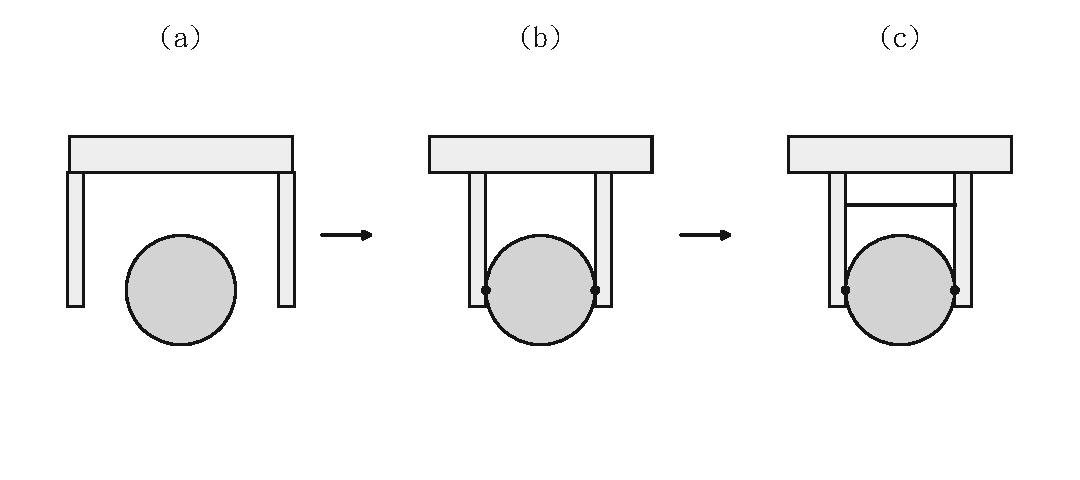
\includegraphics[width=0.98\textwidth]{figsrc/ch03/grasp_state_transition.pdf}
    \caption{接近、閉爪確認與抓持成立之狀態轉移}
    \label{fig:ch3_grasp_state_transition}
\end{figure}

% ==================================================
% 3.6.2 門與抽屜之機構約束建模
% ==================================================
\subsection{門與抽屜之機構約束建模}
\label{subsec:articulated_object_constraints}

令 $\eta$ 為被操作物件的機構座標，$ {}^{W}T_H(\eta)$ 為把手位姿。抓持成立時，由當下物件估計與機器人實測構型建立固定抓持變換：
\begin{equation}
    \begin{aligned}
        {}^{H}T_E
        &=\left({}^{W}T_H(\eta_b)\right)^{-1}
          {}^{W}T_E(\chi_b),\\
        {}^{W}T_E(\chi)
        &={}^{W}T_H(\eta)\,{}^{H}T_E.
    \end{aligned}
    \label{eq:ch3_grasp_closed_chain}
\end{equation}
其中 $\chi_b$ 與 $\eta_b$ 為綁定時刻的構型及機構座標。第二式為抓持後的閉鏈相容關係，底盤與手臂需共同維持末端相對把手的位姿。

對旋轉門，令 $h$ 為鉸鏈軸上一點，$a_h$ 為世界座標中的單位旋轉軸，其方向依門角正向定義。由起始門角 $\phi_0$ 對應的把手位姿，可得
\begin{equation}
    \begin{aligned}
        p_H(\phi)
        &=h+R_{a_h}(\phi-\phi_0)(p_{H,0}-h),\\
        R_H(\phi)
        &=R_{a_h}(\phi-\phi_0)R_{H,0}.
    \end{aligned}
    \label{eq:ch3_revolute_handle_model}
\end{equation}
其中 $R_{a_h}$ 為繞軸 $a_h$ 的旋轉矩陣。開門與關門分別依目標門角更新參考；回程操作前重新估計門扇開度，以處理放手後的門角變化。

% ==================================================
% 3.6.2 開門前後之門扇、底盤與手臂構型
% ==================================================
不同門角下的協同構型如\cref{fig:ch3_door_operation_sequence}所示。把手繞鉸鏈運動時，底盤位置與手臂構型配合調整，並維持式\eqref{eq:ch3_grasp_closed_chain}所定義的抓持相對位姿。

\begin{figure}[htbp]
    \centering
    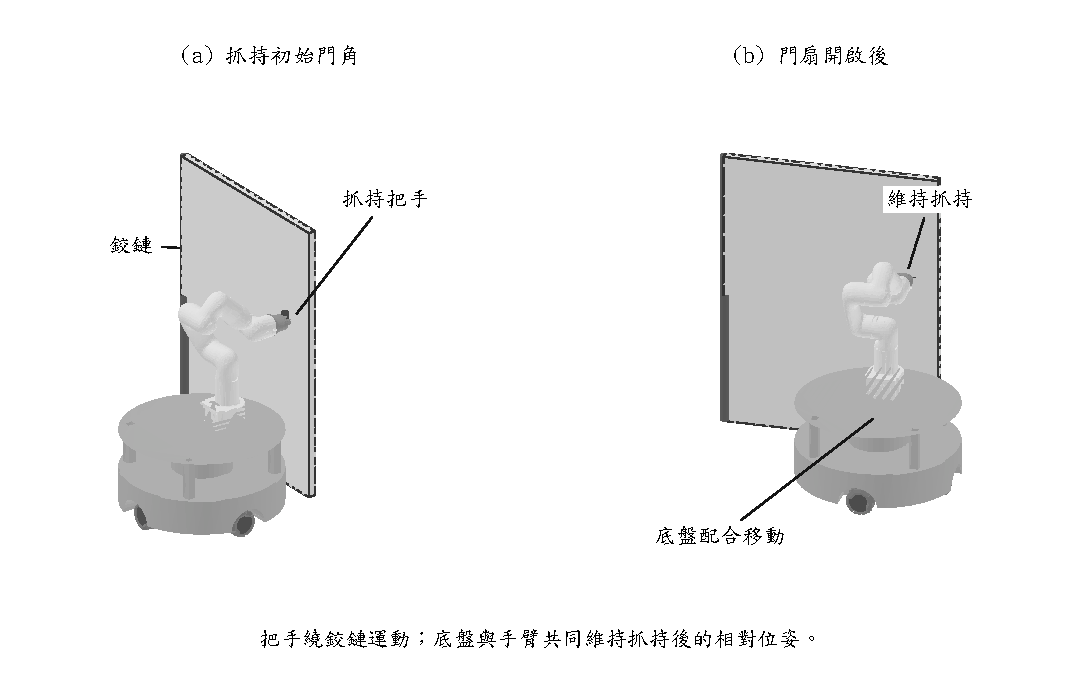
\includegraphics[width=0.98\textwidth]{figsrc/ch03/door_operation_sequence.pdf}
    \caption{開門前後之門扇、底盤與手臂構型}
    \label{fig:ch3_door_operation_sequence}
\end{figure}

對平移抽屜，令 $a_d$ 為拉出方向，$d$ 為相對初始位置的位移，則
\begin{equation}
    p_H(d)=p_{H,0}+d a_d,
    \qquad R_H(d)=R_{H,0}.
    \label{eq:ch3_prismatic_handle_model}
\end{equation}
拉開與推回依位移參考的方向處理，並共同更新底盤與末端參考。物件機構參數、有效行程及家具幾何屬於已知模型或觀測後更新的資訊，實驗中分別揭露其來源。

% ==================================================
% 3.6.2 抽屜拉出前後之滑軌位移與全身構型
% ==================================================
抽屜拉出前後的機構位移與全身構型如\cref{fig:ch3_drawer_operation_sequence}所示。抽屜沿滑軌平移並保持機構姿態，底盤與手臂則依操作進度更新參考，以維持抓持及所需的運動空間。

\begin{figure}[htbp]
    \centering
    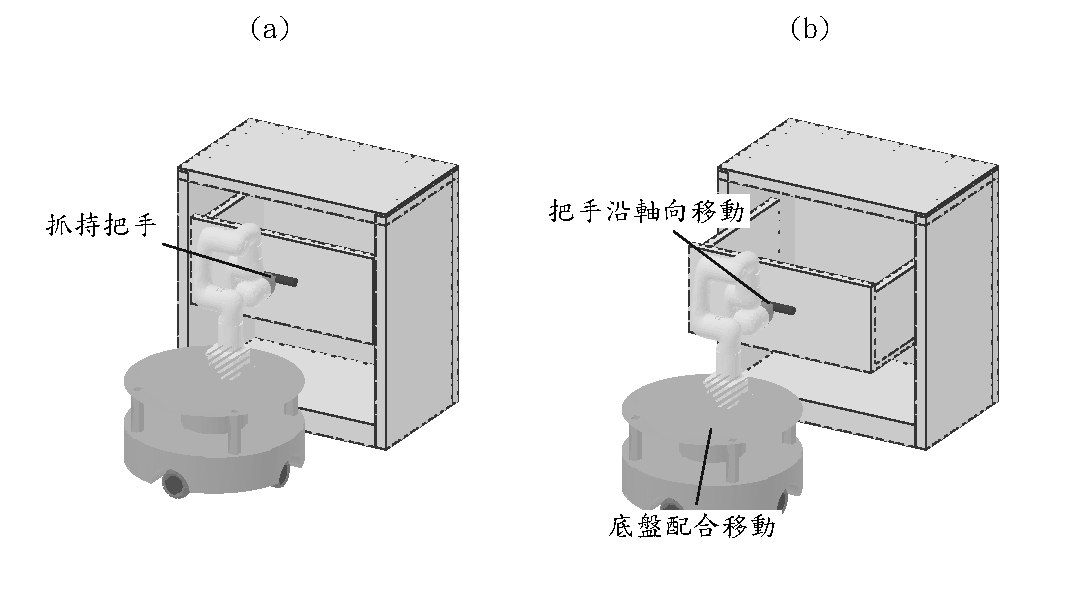
\includegraphics[width=0.98\textwidth]{figsrc/ch03/drawer_operation_sequence.pdf}
    \caption{抽屜拉出前後之滑軌位移與全身構型}
    \label{fig:ch3_drawer_operation_sequence}
\end{figure}



開門階段以把手機構產生末端目標，並可在選定預測步加入閉鏈位姿容許範圍。沿用式\eqref{eq:ch3_tcp_affine_residual}的局部近似，限制為
\begin{equation}
    -\epsilon_c
    \leq r_{0,i|k}-L_{i,k}\mathbf U_k
    \leq\epsilon_c,
    \qquad i\in\mathcal I_c,
    \label{eq:ch3_contact_pose_tube}
\end{equation}
其中 $\epsilon_c$ 分別包含位置與姿態各分量的容許量，$\mathcal I_c$ 為啟用的預測步集合。此限制與底盤、手臂的輸入共同出現在同一 QP 中。

各操作階段依配置採用機構相容參考、QP 限制及執行端幾何核對。抽屜平移與共轉關門的限制實現方式分別說明，不將所有階段視為啟用相同的硬限制。轉動門扇及被操作物件的回波例外，須與專用機構、環境淨空檢查共同啟用，並記錄其適用範圍。


% ==================================================
% 3.6.3 持物運送與收納之運動參考
% ==================================================
\subsection{持物運送與收納之運動參考}
\label{subsec:carrying_storage_reference}

物件抓持成立後，操作目標可由世界固定改為相對底盤的抬升與保持。令 $ {}^{B}T_E^{d}$ 為相對底盤的目標，則其世界位姿為
\begin{equation}
    {}^{W}T_E^{d}
    ={}^{W}T_B\,{}^{B}T_E^{d},
    \qquad
    {}^{B}T_E(q_a)
    ={}^{B}T_A\,{}^{A}T_E(q_a).
    \label{eq:ch3_base_relative_carry_target}
\end{equation}
在相對模式中，追蹤殘差直接由 $ {}^{B}T_E(q_a)$ 與 $ {}^{B}T_E^{d}$ 計算。由於目標與實際末端皆隨底盤作相同剛體運動，其對底盤誤差的局部微分相互抵消，對增廣狀態的幾何映射為
\begin{equation}
    \mathcal J_{E,i}^{\mathrm{rel}}
    =
    \begin{bmatrix}
        \mathbf 0_{6\times3}
        &{}^{B}J_{A,i}
        &\mathbf 0_{6\times6}
    \end{bmatrix}.
    \label{eq:ch3_relative_task_augmented_jacobian}
\end{equation}
因此，持物任務以相對構型維持物件位置，導航則繼續調整底盤運動。相對模式的殘差與雅可比需共同更新，以符合式\eqref{eq:ch3_base_relative_carry_target}的座標關係。

抬升、退出家具、移至收納區及收臂依階段產生參考，並檢查手臂、持物與家具的淨空。住宅整合任務將茶几圓柱及抽屜內的筆狀代理物依序放入車尾收納盒，確認連接解除與釋放後，再轉入後續操作。收納後持續承接關閉抽屜、回程推門通行、關門及返回起點等階段；較早的直接持物返回實驗依其原流程另行比較。

% ==================================================
% 3.6.3 相對底盤目標下之持物運送與構型保持
% ==================================================
相對底盤目標下的運送關係如\cref{fig:ch3_base_relative_carrying}所示。手臂維持相對底盤的末端構型時，物件在世界座標中的位置隨底盤一起改變。此關係由式\eqref{eq:ch3_base_relative_carry_target}建立，與前述世界固定操作目標分別處理。

\begin{figure}[htbp]
    \centering
    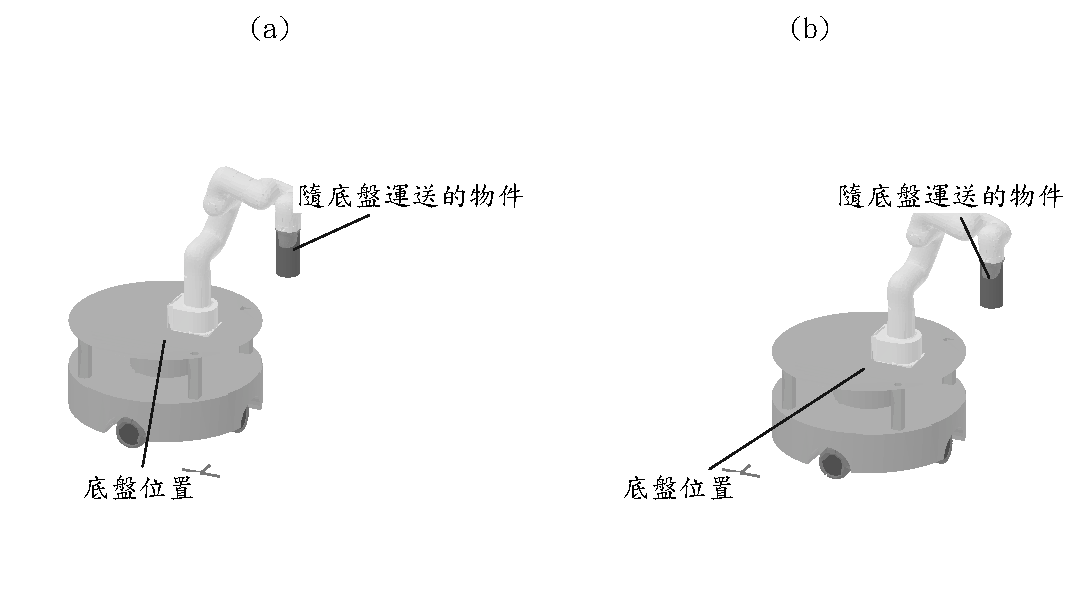
\includegraphics[width=0.98\textwidth]{figsrc/ch03/base_relative_carrying.pdf}
    \caption{相對底盤目標下之持物運送與構型保持}
    \label{fig:ch3_base_relative_carrying}
\end{figure}

% ==================================================
% 3.6.4 任務階段切換與控制狀態延續
% ==================================================
\subsection{任務階段切換與控制狀態延續}
\label{subsec:task_transition_continuity}

任務層管理導航、接近、閉爪確認、機構操作、退出、通行、取物與返回等階段，各階段更新底盤參考、末端目標、權重與啟用限制。轉移條件依觀測、位姿誤差、抓持證據、機構進度及執行端回報判定；時間條件用於軌跡參數化、確認區間及逾時處置。

切換時承接實際關節位置、位置設定點、在途命令、最近放行輸入及模型偏置，並保留可沿用的初始控制序列。新的接近參考由切換時實際相對位姿建立；抓持成立後再依式\eqref{eq:ch3_grasp_closed_chain}建立機構關係。狀態延續使各任務可使用共用全身控制核心，同時維持實際命令的時間順序。

當新階段尚未取得有效目標或未通過交接檢查時，執行端依目前已接受的控制段與停止備援處理。任務切換、求解接受與實際生效分別記錄，以供第四章分析動作接續與非必要等待。
